\chapter{Análisis de Resultados}

Al comparar los resultados obtenidos al construir los mapas de radiación solar de Landsat  con lo de MODIS se puede observar gran similitud,
la manera de establecer relación entre los datos es mediante un análisis de correlación y coeficiente de determinación entre los mapas resultantes 
con los datos de Landsat7 y MODIS. Se tomo los mapas por años del 2005 al 2014  como lo muestra la tabla~\ref{tab:landsatvsmodisanio}, por meses y el 
mapa general ver tabla~\ref{tab:landsatvsmodismes}

Adicionalmente se muestra resultados de datos reales reportados por las estaciones y se los compara con la serie de tiempo construida a partir de imágenes satelitales
MODIS, los resultados obtenidos permiten concluir que la serie de tiempo de radiación solar construida para todo el departamento de Nariño es fiable y puede servir 
como punto de referencia para varios estudios que contemplen la temática.
\begin{table}[H]
\centering
\begin{tabular}{ >{\arraybackslash}m{5cm} >{\centering\arraybackslash}m{3cm}}
\hline
Estación & $R^2$ \\
\hline \hline
Estación Mosquera&  86,57 \% \\
\hline
Estación Ricaurte & 90,33 \%\\
\hline
Granja Barbacoas & 74,09 \%\\
\hline
Granja Betania & 84,64 \%\\
\hline
Granja Buesaco & 76,55 \%\\
\hline
Granja Catambuco & 60,82 \%\\
\hline
Granja La Cruz & 91,26 \%\\
\hline
Granja Obonuco & 71,52 \%\\
\hline
Granja Pupiales & 90,47 \%\\
\hline
Granja San Lorenzo  & 65,11 \%\\
\hline
Granja Santa Barbara & 81,27 \%\\
\hline
\end{tabular}
\caption{Resultado Análisis de Datos para Radiación Solar Reporte Estaciones Vs Serie de Tiempo MODIS.}
\label{tabla:validacione}
\end{table}

\begin{table}[H]
\label{tab:landsatvsmodisanio}
\centering
\scalebox{1}{
\begin{tabular}{c c c}
\toprule
Map &  COR & R2 \\
\midrule
2005 & 0.85594 & 0.73263 \\
\hline
2006 & 0.90754 & 0.82363  \\
\hline
2007 & 0.92884 & 0.86275 \\
\hline
2008 & 0.90594 & 0.82073  \\
\hline
2009 & 0.89443 & 0.80000  \\
\hline
2010 & 0.88594  & 0.78488  \\
\hline
2011 & 0.88233  & 0.77851  \\
\hline
2012 & 0.92056  & 0.84743  \\
\hline
2013 & 0.92982  & 0.86456  \\
\hline
2014 & 0.93167 & 0.86800  \\
\bottomrule
\end{tabular}}
\caption{Análisis Datos Anuales de MODIS vs Landsat 7}
\end{table}

\begin{table}[H]
\label{tab:landsatvsmodismes}
\centering
\scalebox{1}{
\begin{tabular}{c c c}
\toprule
Map &  COR & R2 \\
\midrule
January & 0.89182 & 0.79535 \\
\hline
February & 0.89131 & 0.79444 \\
\hline
March & 0.90943 & 0.82706 \\
\hline
April & 0.90930 & 0.82683 \\
\hline
May & 0.91770 & 0.84218 \\
\hline
June & 0.90244 & 0.81439 \\
\hline
July & 0.90434 & 0.81783 \\
\hline
August & 0.91527 & 0.83772 \\
\hline
September & 0.91810 & 0.84290 \\
\hline
October & 0.92340 & 0.85266 \\
\hline
November & 0.87242 & 0.76111 \\
\hline
December & 0.86934 & 0.75576 \\
\hline
General & 0.94179 & 0.88696 \\
\bottomrule
\end{tabular}}
\caption{Análisis Datos Mensuales de MODIS vs Landsat 7}
\end{table}
\newpage
\chapter{Análisis de Patrón y Nubes en un punto Específico}
Los patrones identificados en la serie de tiempo de los mejores 300 puntos de radiación dentro departamento de Nariño permiten determinar acontecimiento 
frecuentes respecto a los dias en que se presenta mayor o menor radiación solar, por ejemplo para el punto (0.97067,-77.84763) Figura~\ref{fig:pp}, se 
identificó el patrón ['8','1','7','8','6','8','8','8','8','8'] el significado de este patrón esta representado en la tabla ~\ref{tab:pats}, este patrón 
se presentó 1320 veces y permite concluir que de los 10 dias de radiación hay 7 dias en los cuales se presenta radiación superior a 233.5 W/m2 y se puede 
garantizar que este punto es una zona con buena radiación solar, esta información es necesaria para instalar plantas energéticas a base de paneles solares 
siempre que la frecuencia de nubes sea baja.
\begin{figure}[htbp]
  \centering 
  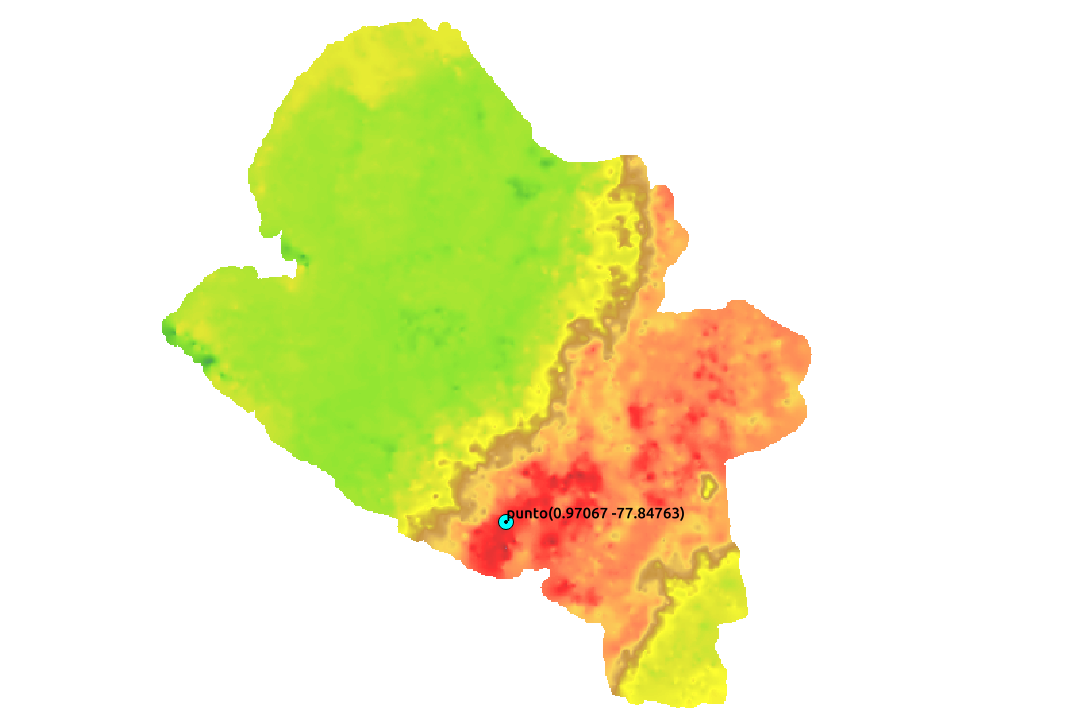
\includegraphics[scale=0.55]{pictures/pp.png}
  \caption{ Plataforma GEOAlternar- mapas energéticos del departamento de Nariño}
  \label{fig:pp}
\end{figure}

\begin{table}[H]
\label{tab:pats}
\centering
\begin{tabular}{>{\centering\arraybackslash}m{2cm} >{\centering\arraybackslash}m{3cm} >{\centering\arraybackslash}m{3cm} >{\centering\arraybackslash}m{5cm}}
\hline
N. Dias & Bin BD(Patrón) &  Color & Rango \\
\hline \hline
1 & 8 & 
\includegraphics[width=3mm]{pictures/suns/so8.png}  & 233.534 - x>233.534 \\
\hline
2 & 1 & 
\includegraphics[width=3mm]{pictures/suns/so1.png} & 0 - 195.985\\
\hline
3 & 7 & 
\includegraphics[width=3mm]{pictures/suns/so7.png} & 228.426 - 233.534 \\
\hline
4 & 8 & 
\includegraphics[width=3mm]{pictures/suns/so8.png} & 233.534 - x>233.534 \\
\hline
5 & 6 & 
\includegraphics[width=3mm]{pictures/suns/so6.png} & 205.954 - 228.426 \\
\hline
6 & 8 & 
\includegraphics[width=3mm]{pictures/suns/so8.png} & 233.534 - x>233.534 \\
\hline
7 & 8 & 
\includegraphics[width=3mm]{pictures/suns/so8.png} & 233.534 - x>233.534 \\
\hline
8 & 8 & 
\includegraphics[width=3mm]{pictures/suns/so8.png} & 233.534 - x>233.534 \\
\hline
9 & 8 & 
\includegraphics[width=3mm]{pictures/suns/so8.png} & 233.534 - x>233.534 \\
\hline
10 & 8 & 
\includegraphics[width=3mm]{pictures/suns/so8.png} & 233.534 - x>233.534 \\
\hline
\end{tabular}
\caption{Análisis de Patrón en el punto (0.97067,-77.84763)}
\end{table}
La probabilidad de que en el punto (0.97067,-77.84763) se presenten nubes es de 28\% en cuanto al cambio en el tiempo se puede observar en la tabla ~\ref{tab:ncy}
y la tabla ~\ref{tab:ncm}, esta información es muy importante debido a que la presencia constante de nubes termina afectando la producción energética a base
de paneles solares y así poder plantear una solución alternativa para generar energía.
 
\begin{table}[H]
\label{tab:ncy}
\centering
\begin{tabular}{>{\centering\arraybackslash}m{2cm} >{\centering\arraybackslash}m{3cm} }
\hline
Año&Probabilidad \\
\hline\hline
2005&26.1475\% \\
\hline
2006&26.8242\% \\
\hline
2007&31.5918\% \\
\hline
2008&31.1175\% \\
\hline
2009&29.7392\% \\
\hline
2010&26.9092\% \\
\hline
2011&26.0167\% \\
\hline
2012&28.0983\% \\
\hline
2013&28.2908\% \\
\hline
2014&26.67\% \\
\hline
2015&26.9967\% \\
\hline
\end{tabular}
\caption{Nubes en el punto (0.97067,-77.84763)}
\end{table}

\begin{table}[H]
\label{tab:ncm}
\centering
\begin{tabular}{>{\centering\arraybackslash}m{2cm} >{\centering\arraybackslash}m{3cm} }
\hline
Mes& Probabilidad \\
\hline \hline
January&29.676\% \\
\hline
February&31.9309\% \\
\hline
March&35.7782\% \\
\hline
April&25.7582\% \\
\hline
May&27.5673\% \\
\hline
June&31.5164\% \\
\hline
July&28.4464\% \\
\hline
August&26.3918\% \\
\hline
September&27.2718\% \\
\hline
October&23.225\% \\
\hline
November&21.667\% \\
\hline
December&26.129\% \\
\hline
\end{tabular}
\caption{Nubes en el punto (0.97067,-77.84763)}
\end{table}

